
\chapter{Aufgabe D3}

\section{Simulink-Modell}
Die nachfolgenden Abbildungen zeigen das Simulink-Modell zur Berechnung der Distanzen der einzelnen Räder.\\
Das Modell in \autoref{fig:drivingdistances1} hat die vier Geschwindigkeiten (in km/h) der Räder als Eingänge. Diese werden mit dem \glqq From Workspace"' Block mit ihrer zugehöhrigen Referenzzeit tv in das Model importiert.\\
Danach werden sie in m/s umgerechnet und integriert, um die Strecke zu erhalten. \\
Zur Simulation wird ein FixedStep von 0.01 mit dem ode3-Solver verwendet. Der ode-Solver wurde durch die SImulink \glqq automatic solver selection"' ausgewählt.
\begin{figure}[h!]
	\centering
	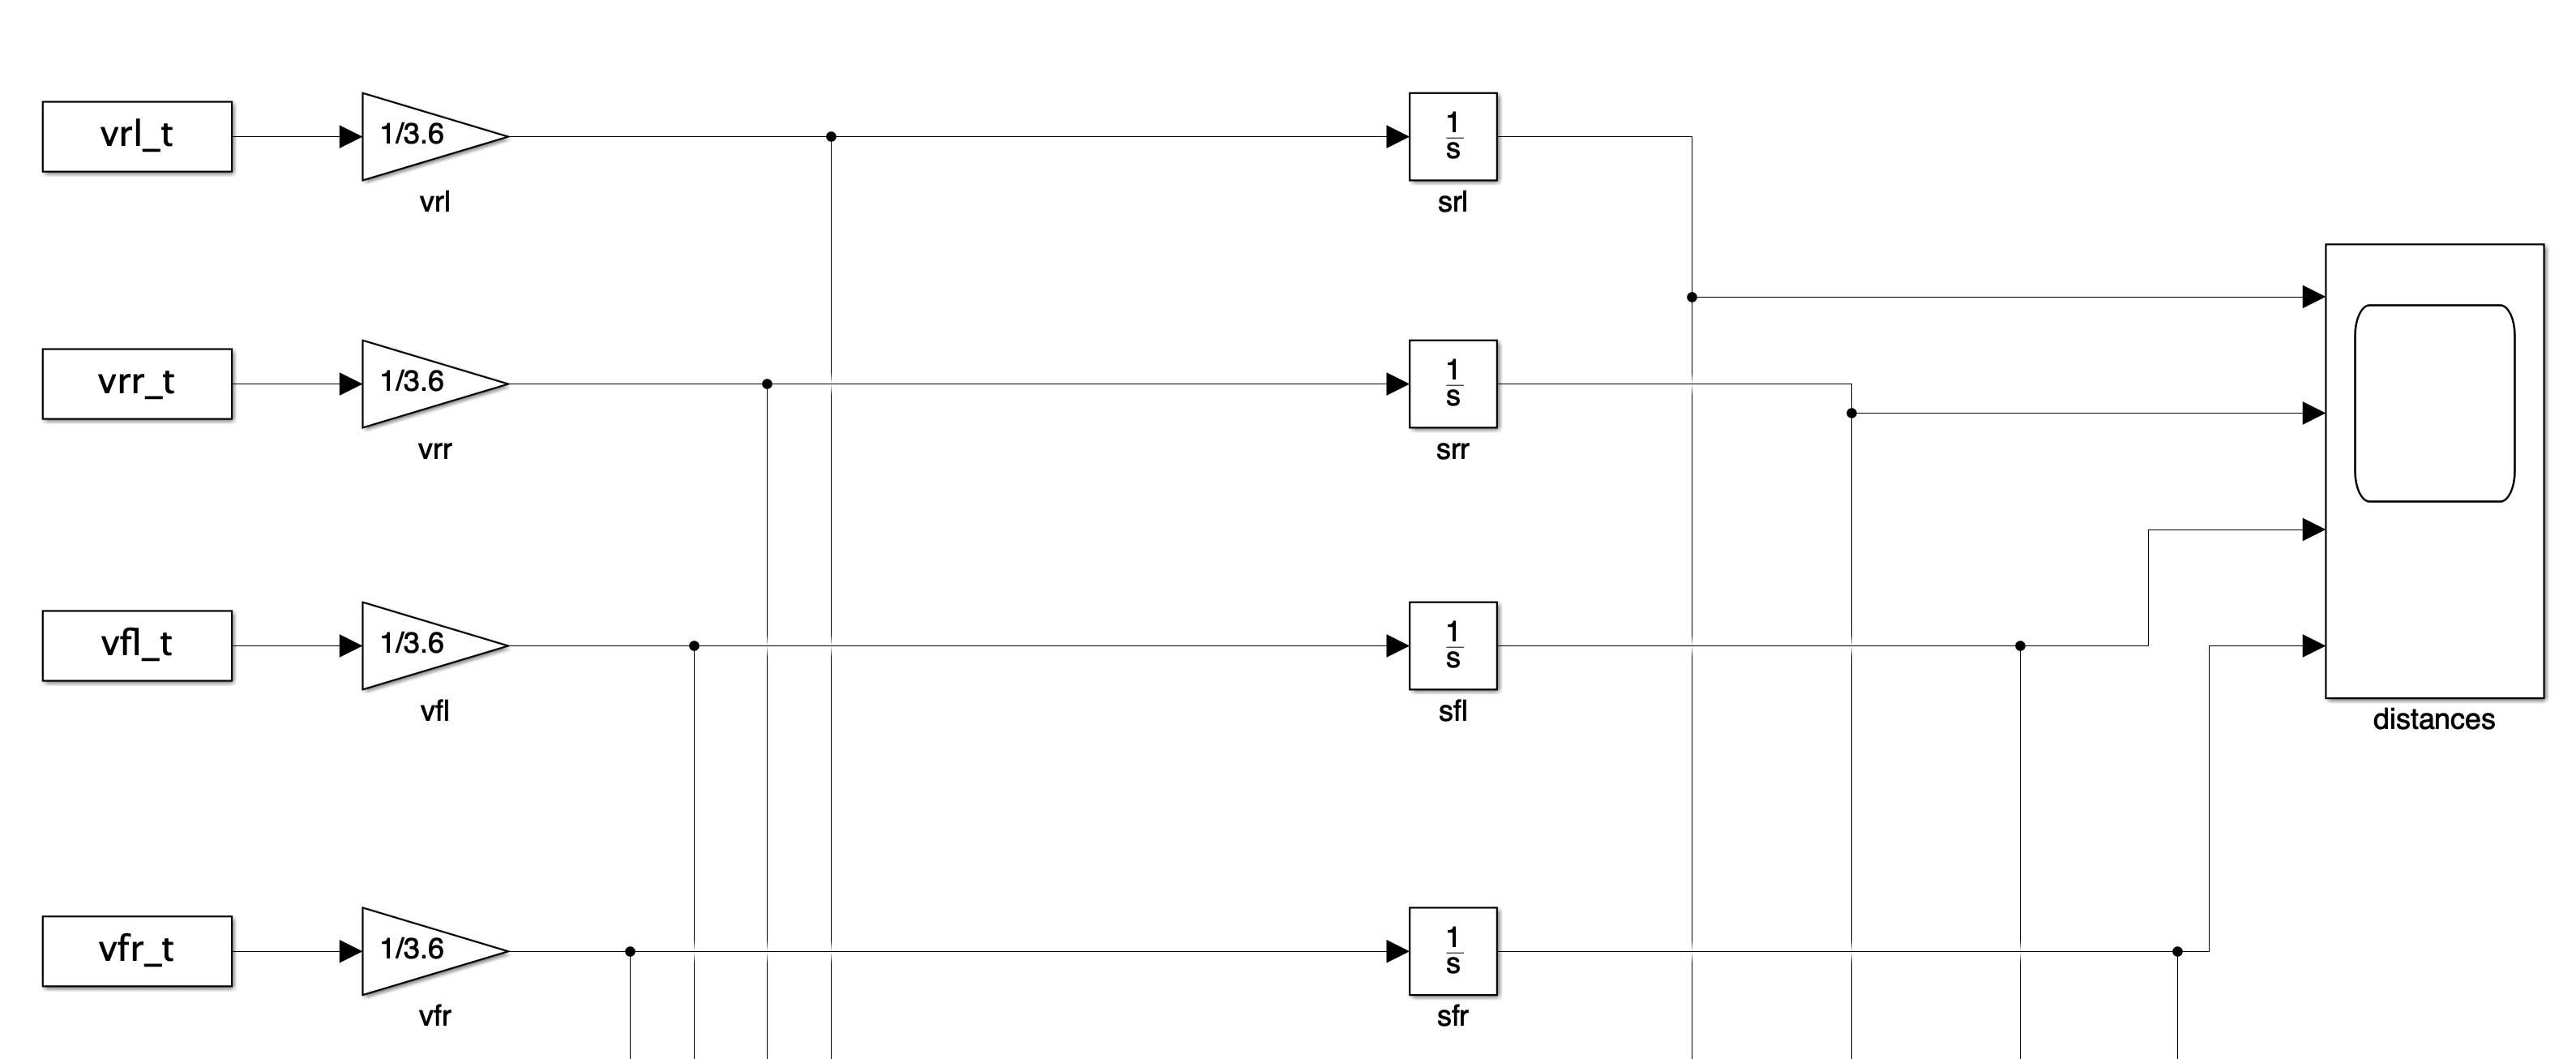
\includegraphics[width=1\linewidth]{../Graphiken/DrivingDistances1}
	\caption{Tire Driving distances}
	\label{fig:drivingdistances1}
\end{figure}
Das Ergebnis der Integration sind die Distanzen der einzelnen Reifen, die gegenüber der Zeit aufgetragen sind.\newpage
\begin{figure}[h!]
	\centering
	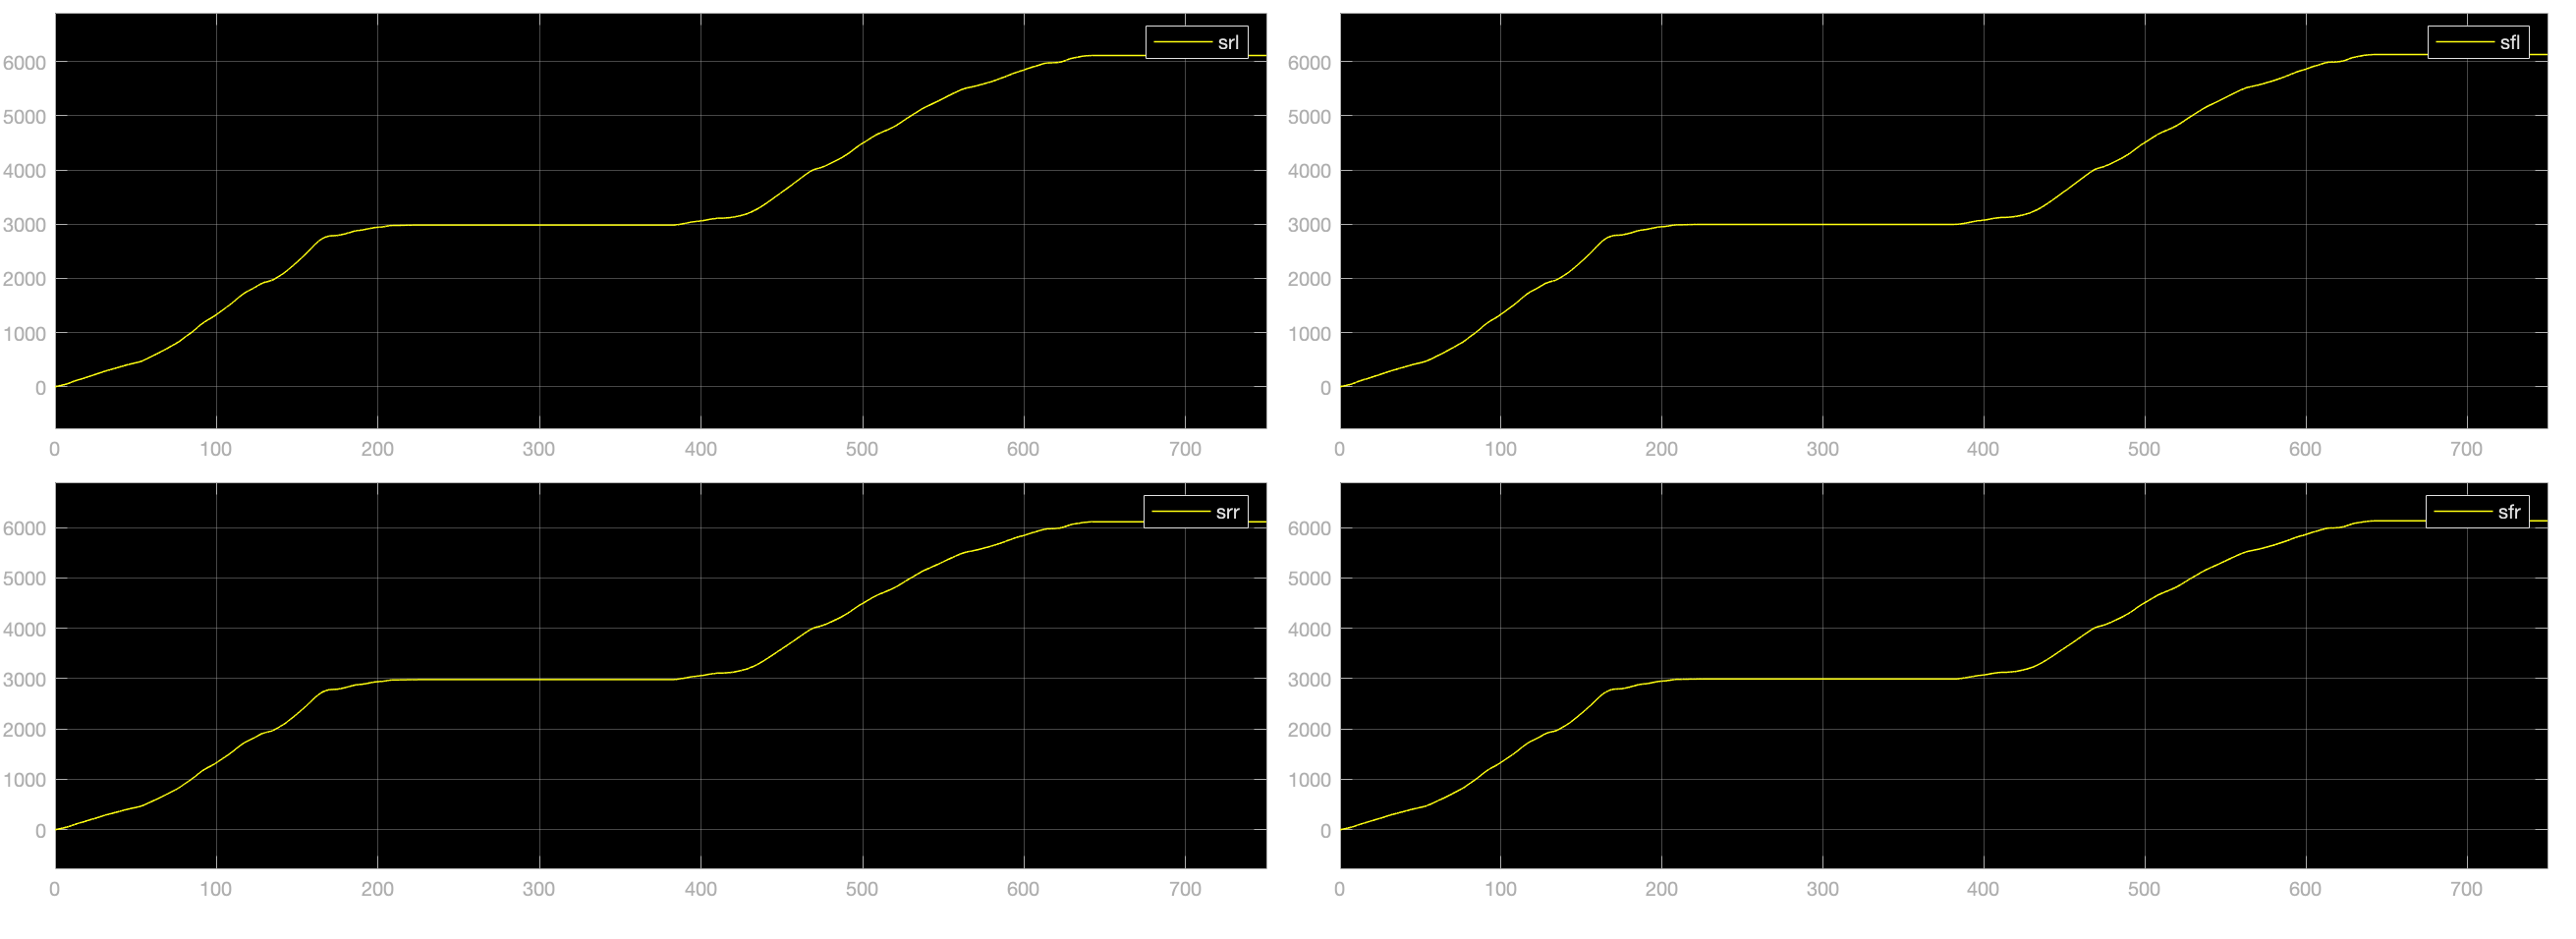
\includegraphics[width=1\linewidth]{../Graphiken/DrivingDistances}
	\caption{Tire Driving distances plot}
	\label{fig:drivingdistances}
\end{figure}

Zur Überprüfung ob es Imbalancen in den Daten gibt wird das Modell wie in \autoref{fig:TireSImCurves} zu sehen ist erweitert.
Der Mittelwert der vier integrierten Distanzen gilt als Referenzwert, ob ein Reifendruckabfall vorliegt. Die Berechnung ist ebenfalls im erweiterten Modell \autoref{fig:TireSImCurves} zusehen. Anschließend wird die prozentuale Abweichung vom Einzelsignal zum Mittelwert berechnet, weicht die Abweichung um mehr als 0.5\% ab handelt es sich um einen Reifendruckabfall. Die Berechnung ist in \autoref{fig:abweichung} dargestellt. 
\begin{figure}[H]
	\centering
	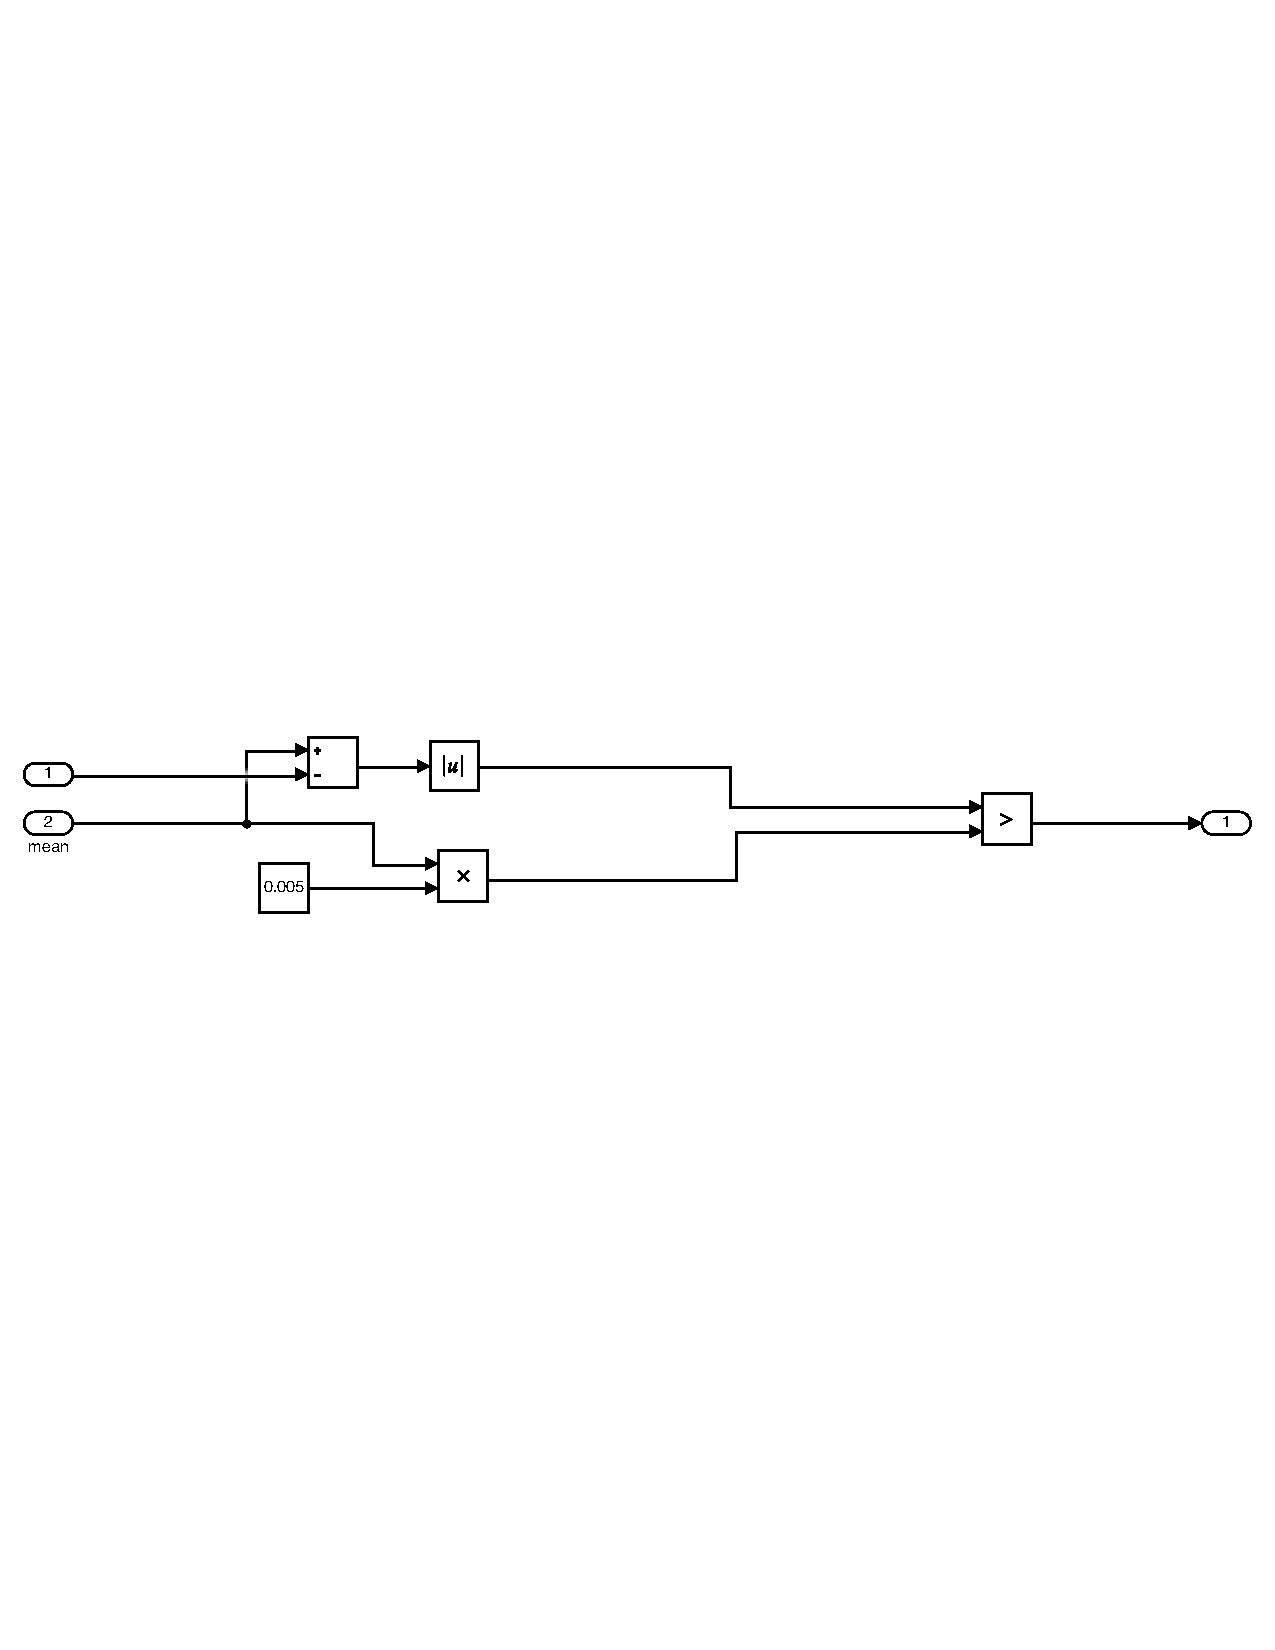
\includegraphics[width=1\linewidth]{../Graphiken/PDFSplit/3_PDFsam_SebastianTireSim2.pdf}
	\caption{Prozentuale Abweichung nach R2}
	\label{fig:abweichung}
\end{figure}
Damit die Messungen nicht durch Rauschen im Geschwindigkeitssignal verfälscht werden, wird das integrierte Signal zur Messung verwendet. Durch die Integration wird das kurzzeitiges Rauschen sozusagen gemittelt, sodass es die Messung nicht verfälscht. Damit jedoch ein Reifendruckabfall nicht untergeht, da das bereits integrierte Signal zu groß ist wird in Deltas von 10 Sekunden gemessen.\\
Dazu wird der  \glqq Transport Delay"' Block genutzt der das Signal um eine beliebige Zeit (hier 10 Sekunden) verzögert. Das Verzögerte Signal kann dann vom Originalsignal abgezogen werden, sodass ausschließlich das Integral der letzten 10 Sekunden betrachtet wird.\footnote{In den ersten 10 Sekunden, ist der Output des Transport Delays 0, sodass in den 10 Sekunden Rauschen durchaus die Messungen verfälschen kann. Deswegen wird der Output des Transport Delays in den ersten 10 Sekunden manuell auf -1000 gesetzt, sodass die Messung in den ersten 10 Sekunden bewusst so manipuliert wird, dass es keine Imbalancen gibt }\\
Die Berechnungen für die Abweichungen werden für jeden Reifen einzeln berechnet und anschließend, wie in \autoref{fig:TireSImCurves} zu sehen, verodert, um ein Überblick über das Gesamtsystem zu erhalten.\\


\begin{figure}[H]
	\centering
	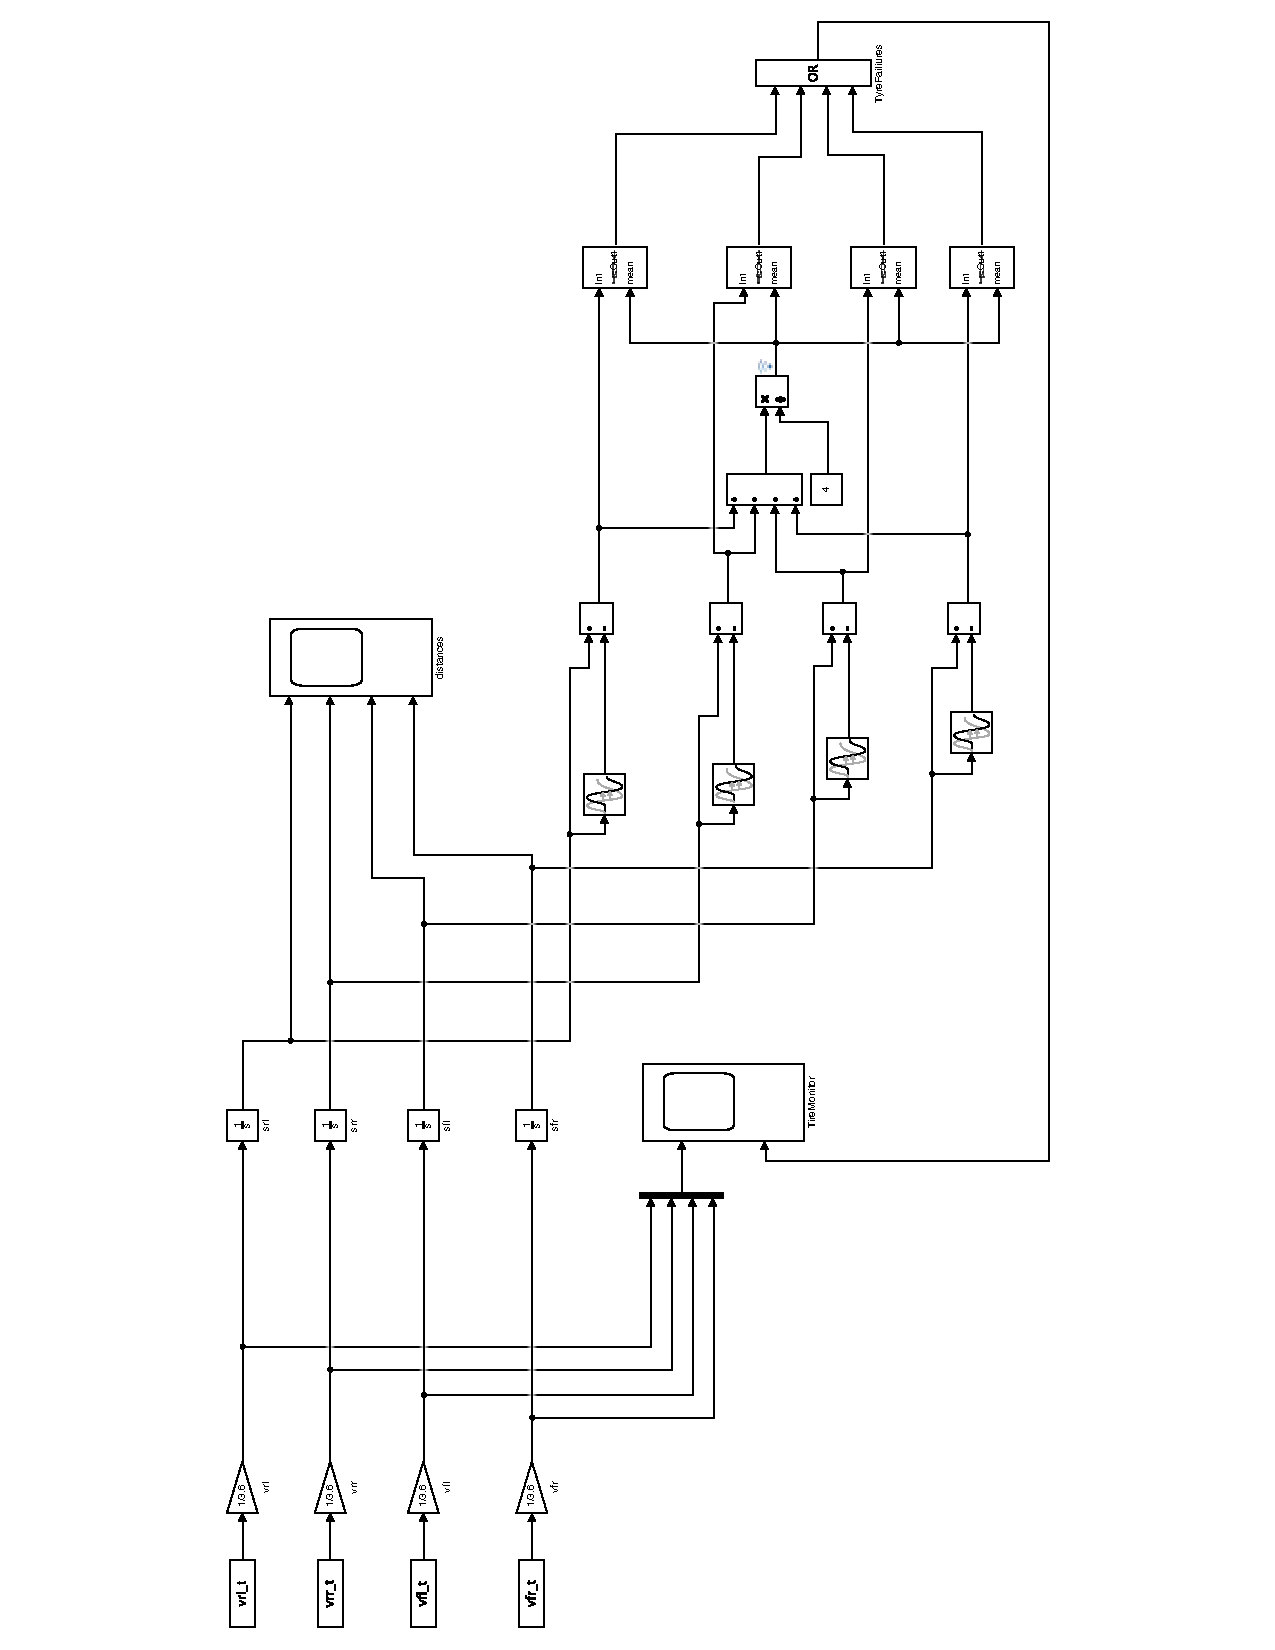
\includegraphics[height=0.95\textheight]{../Graphiken/TireSimCurvesLandscape.pdf}
	\caption{Simulink Tire Distance Model with Curves Data}
	\label{fig:TireSImCurves}
\end{figure}


Für die Kurvenfahrt entsteht die folgende Datenaufzeichnung über die Reifendruckabweichungen.
\begin{figure}[H]
	\centering
	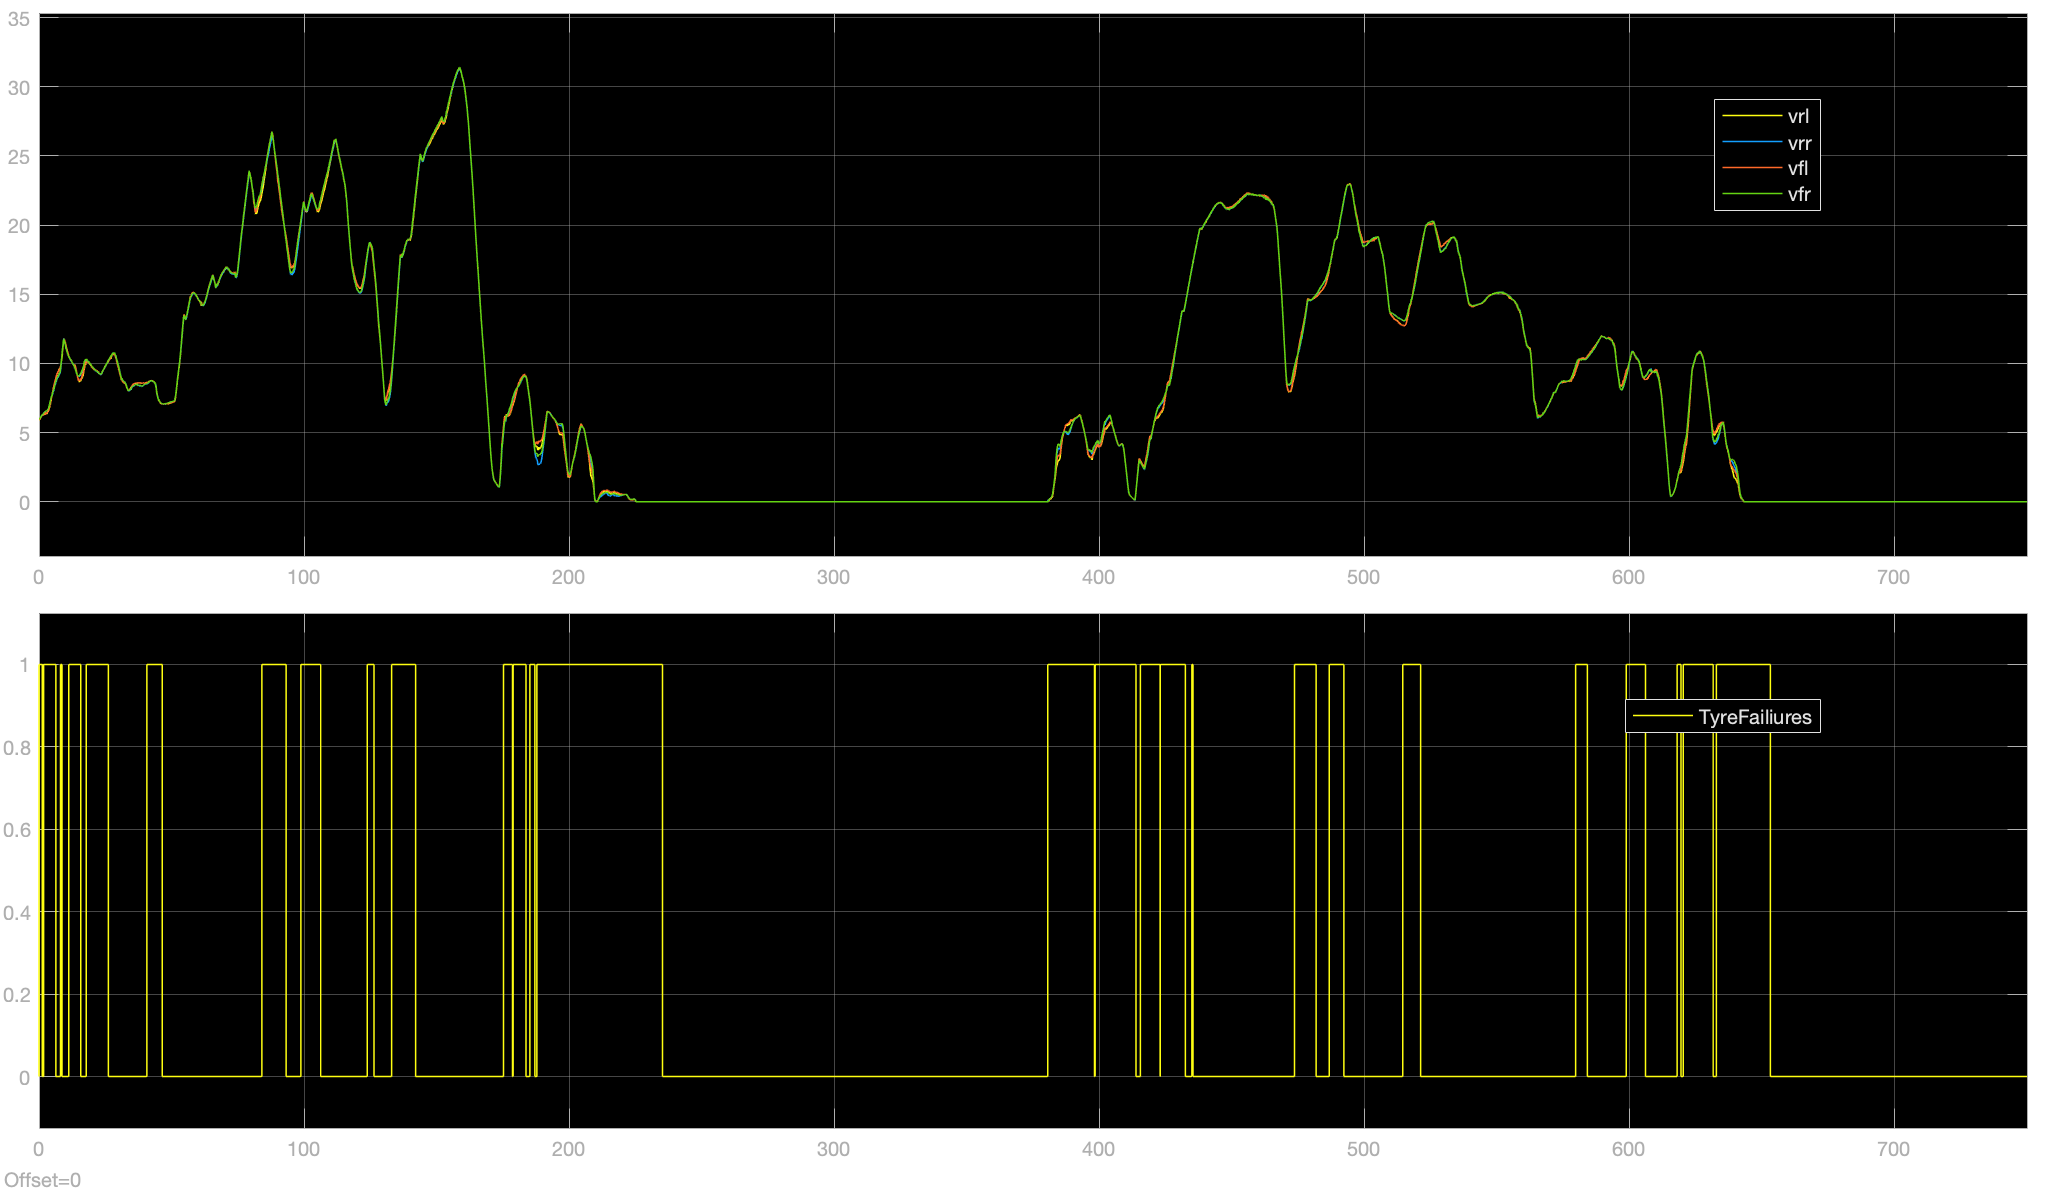
\includegraphics[width=0.95\linewidth]{../Graphiken/CurvesTireMonitor.png}
	\caption{Tire Monitor für Kurvenfahrt}
\end{figure}
Ein Wert von 1  entspricht einer Beobachtung einer Imbalance und ein Wert von 0 entspricht keiner Anomalie.








	
	

	
	
	
	